\documentclass[a4paper, 12pt, english]{article}

% \usepackage[portuges]{babel}
\usepackage[utf8]{inputenc}
\usepackage{amsmath,amssymb}
\usepackage{graphicx}
\usepackage{subfig}
\usepackage[colorinlistoftodos]{todonotes}

\usepackage{indentfirst}
\usepackage{verbatim}
\usepackage{textcomp}
\usepackage{gensymb}

\usepackage{relsize}

\usepackage{lipsum}% http://ctan.org/pkg/lipsum
\usepackage{xcolor}% http://ctan.org/pkg/xcolor
\usepackage{xparse}% http://ctan.org/pkg/xparse
\NewDocumentCommand{\myrule}{O{1pt} O{2pt} O{black}}{%
  \par\nobreak % don't break a page here
  \kern\the\prevdepth % don't take into account the depth of the preceding line
  \kern#2 % space before the rule
  {\color{#3}\hrule height #1 width\hsize} % the rule
  \kern#2 % space after the rule
  \nointerlineskip % no additional space after the rule
}
\usepackage[section]{placeins}

\usepackage{booktabs}
\usepackage{colortbl}%
   \newcommand{\myrowcolour}{\rowcolor[gray]{0.925}}
   
\usepackage[obeyspaces]{url}
\usepackage{etoolbox}
\usepackage[colorlinks,citecolor=black,urlcolor=blue,bookmarks=false,hypertexnames=true]{hyperref} 

\usepackage{geometry}
\geometry{
	paper=a4paper, % Change to letterpaper for US letter
	inner=3cm, % Inner margin
	outer=3cm, % Outer margin
	bindingoffset=.5cm, % Binding offset
	top=2cm, % Top margin
	bottom=2cm, % Bottom margin
	%showframe, % Uncomment to show how the type block is set on the page
}
%*******************************************************************************%
%************************************START**************************************%
%*******************************************************************************%
\begin{document}

%************************************TITLE PAGE**************************************%
\begin{titlepage}
\begin{center}
\textbf{\LARGE Universidade Federal de Alagoas}\\[0.5cm] 
\textbf{\large Instituto de Computação - IC}\\[0.2cm]
\vspace{20pt}
%* \includegraphics{Logo_Utar.png}\\[1cm] *%

\par
\vspace{20pt}
\vspace{20pt}
\vspace{20pt}
\vspace{20pt}
\vspace{20pt}
\vspace{20pt}
\vspace{20pt}
\vspace{20pt}
\vspace{20pt}
\textbf{\Large Aluno: Marcos Gleysson Silva do Nascimento}\\ 
\vspace{15pt}
\myrule[1pt][7pt]
\textbf{\LARGE  Seminário 1}\\
\vspace{15pt}
\textbf{\large Análise e Classificação estatísticas para imagens SAR }\\
\myrule[1pt][7pt]
\vspace{25pt}
\textbf{\large Orientador: Alejandro Frery}\\

% 2. Low Hui Tyen \hspace{45pt} 14AGB06230 \\ % No2

\vspace{45pt}
\end{center}

\par
\vfill
\begin{center}
\textbf{Maceió - AL}\\
\textbf{2017}
\end{center}

\end{titlepage}

%************************************TABLE OF CONTENTS**************************************%

%  %Sumário
%  \newpage
%  \tableofcontents
%  \thispagestyle{empty}
%  %End Sumário

%********************************%
%***********SECTION 1************%
%********************************%
\newpage
\section{Introdução}
A intensificação de estudos na área de Sensoriamento Remoto voltado para os
radares imageadores de abertura sintética (Sinthetic Aperture Radar - SAR) tem
proporcionado, cada vez mais, o melhor entendimento dos mecanismos de dispersão dos
alvos terrestres na faixa de microondas. Desta forma, as aplicações de imagens SAR nos
mais variados campos do conhecimento humano (Geologia, Cartografia, etc.) tornam-se
mais confiáveis, principalmente em regiões onde a obtenção de imagens geradas por
sensores ópticos é muito difícil, devido a fatores climáticos.

Nesse sentido, o radar possui uma clara vantagem sobre sensores ópticos, devido
ao fato de sua capacidade ser praticamente inafetada pela escuridão, pelas nuvens ,
neblina e fumaça. O retroespalhamento do radar é muito sensível a vários parâmetros do
alvo e do sistema. Essa característica fornece informações multidimensionais que podem
ser usadas em áreas importantes como monitoramento agrícola, especialmente se um
radar de alta resolução, como no caso do SAR – Radar de Abertura Sintética – é utilizado.

Cada vez mais os algoritmos de classificação para imagens SAR tornam-se mais
precisos, quando os resultados por eles obtidos são comparados com verdades terrestres.
Essa melhora está diretamente ligada, entre outros fatores, a uma modelagem mais
adequada aos dados SAR, como mostrada em Nezry et al. (1996) e Frery et al. (1997).

Em Vieira (1996) isso fica bem evidente, através do uso das distribuições mais
apropriadas às observações (radiometria) provindas de diferentes classes, utilizadas na
classificação por Máxima Verossimilhança (MaxVer), além da modelagem das classes
(informação contextual) através do algoritmo Iterated Conditional Modes (ICM).

Com o advento de novos sensores, pode-se dispor cada vez mais de um grande
volume de imagens de sensoriamento remoto. Torna-se necessário, pois, processar-se
imagens de forma rápida e obter-se de maneira precisa a informação procurada. Uma das
técnicas mais úteis no processamento de imagens é a da classificação automática na qual
se permite automatizar tarefas associadas à interpretação visual de imagens, diminuindo
assim o tempo entre a aquisição dos dados e a sua análise.

Embora existam várias técnicas de classificação automática de imagens, poucas
delas são adequadas para os problemas particulares que apresentam as imagens SAR. A
maioria dos procedimentos para a análise e classificação de imagens disponíveis em
sistemas comerciais se baseia na hipótese de que os dados sejam normalmente
distribuídos, hipótese rara observada nas imagens SAR. As propriedades estatísticas das
imagens SAR dependem de parâmetros do sistema imageador como também de
parâmetros do alvo a ser imageado.

Verifica-se dessa forma a necessidade de se desenvolver técnicas e procedimentos
estatísticos específicos para análise e classificação de imagens SAR.

%********************************%
%***********SECTION 2************%
%********************************%
\newpage
\section{Modelos Estatísticos para dados SAR}
O modelo multiplicativo é comumente adotado para a explicação do comportamento
estatístico de dados obtidos com radiação coerente, como é o caso das imagens SAR. Este
modelo supõe que o valor observado em cada pixel é a ocorrência de uma variável aleatória Z = X.Y, onde X representa a variável aleatória referente ao retroespalhamento do pulso incidente na superfície terrestre (backscatter) e Y representa a variável aleatória referente ao ruído associado à radiação coerente (speckle). Diferentes distribuições para X e Y acarretam diferentes distribuições para a variável aleatória Z.

Nesse contexto decorre-se do Método Multiplicativo, a distribuição GA que possui
como casos especiais as seguintes distribuições: KA, GA0 e $\Gamma^{1/2}$. Observa-se a GA0 modela bem dados provenientes de áreas extremamente heterogêneas como é o caso de
áreas urbanas, enquanto que as distribuições KA e $\Gamma^{1/2}$. são utilizadas para modelagem de áreas heterogêneas (floresta) e homogêneas (solo exposto, pastagem, culturas agrícolas). O grau de homogeneidade está associado, entre outros fatores, aos parâmetros do sensor.

\subsection{SAR MONOESPECTRAL}
Para explicar o comportamento estatístico desse tipo de dado SAR, o modelo multiplicativo
é bastante empregado, pois tanto o backscatter como o speckle podem ser modelados de
formas diferentes, dependendo do tipo de aplicação (Yanasse, 1991; Yanasse et al., 1995;
Vieira, 1996; Frery et al., 1997). Dependendo dos diferentes tipos de detecção, linear
(imagem em amplitude) e quadrática (imagem em intensidade), e das diferentes regiões
imageadas, as distribuições associadas a X e Y variam, produzindo diferentes distribuições
para Z (Ulaby e Dobson, 1989; Frery et al., 1997). Distribuições decorrentes do modelo
multiplicativo para imagens SAR monoespectrais em intensidade possuem as variáveis
aleatórias X e Y , associadas a esse modelo com o subscrito “I”.

Sob certas condições (Ulaby et al, 1986; Goodman, 1963) pode-se supor que o speckle
possui uma distribuição G(n,n) , onde n é o número equivalente de looks3 (nel). Várias
distribuições podem ser utilizadas para o backscatter, visando a modelagem para diferentes
tipos de classes e seus diferentes graus de homogeneidade. Por exemplo, para alguns
parâmetros do sensor (comprimento de onda, ângulo de incidência, polarização, etc.) uma
pastagem pode ser mais homogênea que floresta, a qual é mais homogênea que áreas
urbanas.

Frery et al. (1997) apresenta a modelagem para o caso geral, considerando que
o backscatter possui uma distribuição Gaussiana Inversa Generalizada. Esta distribuição
possui casos especiais mais simples que têm se mostrado úteis na modelagem de áreas
com diferentes graus de homogeneidade. A modelagem para esses casos especiais possui
a vantagem de tornar mais fácil a estimação dos parâmetros das distribuições.

Na Figura 1 abaixo são apresentadas, para dados em intensidade multi-look (ou n-looks), as
possíveis distribuições associadas a regiões com diferentes graus de homogeneidade,
denominadas aqui de regiões homogêneas, heterogêneas e extremamente heterogêneas.

 \begin{figure}[!ht]
 			\begin{center}
				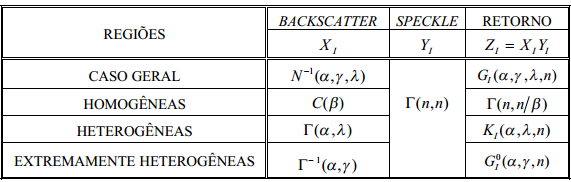
\includegraphics[width=100mm,scale=0.5]{tabela.png}
			\end{center}
       		\caption{\label{Retorno em intensidade para N - Looks}}
 \end{figure}

%********************************%
%***********SECTION 3************%
%********************************%

\section{Classificação por Máxima Verossimilhança}

A classificação por Máxima Verossimilhança (MaxVer) é uma das técnicas de
classificação supervisionada comumente utilizada em dados de Sensoriamento Remoto.
Os principais passos para efetuar esta classificação são:

\begin{itemize}
   \item  Decidir entre os possíveis conjuntos de classes da cobertura terrestre, aquele que
será utilizado para particionar a imagem a ser classificada;
   \item  Associar uma distribuição a cada classe;
   \item Selecionar e retirar amostras de regiões representativas de cada classe na imagem;
   \item Estimar os parâmetros das distribuições associadas a cada classe;
   \item Opcionalmente, pode-se testar o ajuste das distribuições associadas a cada classe;
   \item Classificar a imagem, atribuindo cada pixel da imagem à classe com maior
verossimilhança.
 \end{itemize}

%********************************%
%***********SECTION 4************%
%********************************%

\section{Classificação ICM}

O critério de Máxima Verossimilhança é de maximizar uma função que somente
depende da radiometria observada e do modelo (densidade) escolhido para cada classe.
Esse critério não considera a informação contextual já que supõe que as radiometrias dadas as classes são eventos independentes. Na literatura várias propostas para incorporar
informação contextual, mas a maioria delas leva algoritmos computacionalmente muito
difíceis de serem usados. Em (Frery, 1993) é mostrada uma versão de um algoritmo de
classificação contextual que apresenta alto desempenho e facilidade de uso. Esta técnica,
o algoritmo ICM (Iterated Conditional Modes) foi melhorada em (Vieira, 1996) e aplicada a
várias imagens de radar.

O algoritmo ICM é um método iterativo de refinamento de classificações que consiste
em substituir a classe associada a cada coordenada por aquela classe que maximiza um
certo critério. Esse critério é a distribuição a posteriori da classe, dadas a radiometria
(componente MaxVer) e as classes vizinhas (componente de contexto). A influencia das
classes vizinhas é quantificada por um parâmetro real que é estimado iterativamente
supondo um modelo para distribuição espacial das classes.




\end{document}